\documentclass[a4paper]{report}
\usepackage{amssymb}
\usepackage{amsmath}
\usepackage{graphicx}
\usepackage{lmodern}
\usepackage[T1]{fontenc}
\usepackage{fancyhdr}
\usepackage{lastpage}
\usepackage{geometry}
 \geometry{
 a4paper,
 total={170mm,257mm},
 left=20mm,
 top=20mm,
 }
\graphicspath{{images/}}
\renewcommand{\sfdefault}{phv}
\renewcommand{\familydefault}{\sfdefault}
\title{\huge
{\textbf{Relatório 2}}
 \\
\fontsize{30pt}{36pt}\selectfont{\textbf{O Pêndulo Físico}}
}
\author{
Autores:\\ \ \\
Eduardo Barbosa Jubilado (217494)\\
Gustavo Guimarães de Carvalho (258492)\\
Isabel Shurman Feitoza (218316)\\
Maria Eduarda Teixeira S. Hage (267139) 
}
\date{Setembro, 2023}



\begin{document}

\pagestyle{fancy}
\fancyfoot{}\fancyhead{}
\pagenumbering{arabic}
\maketitle{}
\pagebreak
\fancyhead[C]{Relatório 2 - F 229 2s2023}
\fancyfoot[R]{\thepage}
\section*{Resumo}

\section*{Introdução}
\qquad Neste laboratório iremos utilizar a ideia de movimento pêndular. Como é observado na Figura 1, possuímos um pêndulo simples com uma massa oscilando ao redor de um ponto fixo, preso por um fio de massa desprezível com um comprimento "L" do ponto fixado até o centro de massa do objeto observado. Nesse modelo, podemos perceber que existe a atuação de uma força restauradora devido a força gravitacional que atua no sistema, assim a resultante da força sempre irá apontar para a posição onde o sistema se encontra em equilíbrio, onde em módulo seu valor aumentará à medida que o corpo preso se afasta dessa posição. O movimento é repetido periodicamente e denominamos período (T) como o tempo que esse corpo descreve em um ciclo. 

\begin{figure}[!htb]
    \centering
    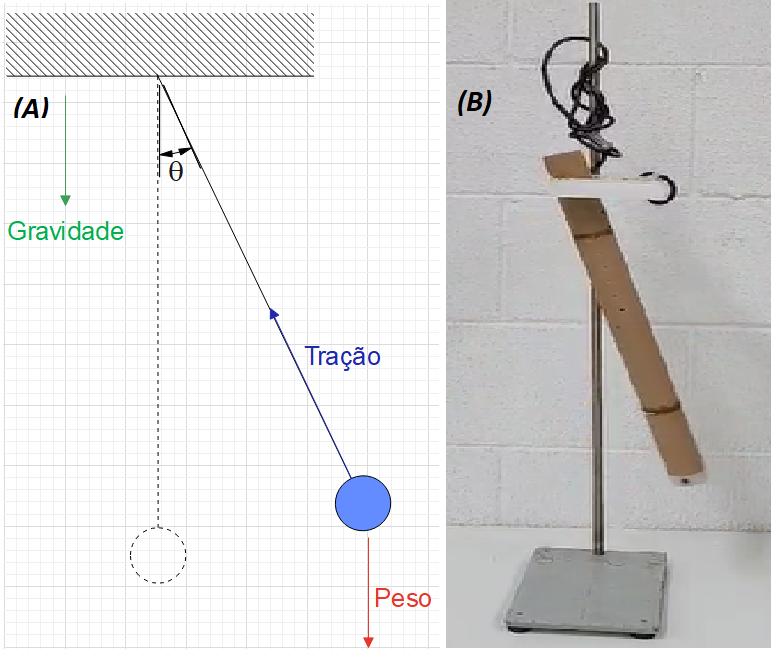
\includegraphics[scale=0.5]{pendulo.png}
    \caption{(A) Diagrama de forças do pêndulo simples incluindo força da gravidade, e (B) experimento montado em laboratório com rolo de papel alumínio, arame e haste de metal.}
    \label{fig:Figura 1}
\end{figure}

\section*{Objetivo}
\qquad O objetivo do experimento é estimar a aceleração da gravidade a partir dos resultados de um pendulo simples em comparação com um pendulo físico. 


\section*{Modelo}
\qquad Podemos escrever uma relação equivalente a segunda lei de Newton através de um sistema de coordenadas polares se acaso quisermos descrever essa relação de movimento para torques através de movimentos pendulares, definindo o centro de massa como referência: 

\begin{equation}
    \sum{\tau_i} =  I\cdot \alpha
\end{equation}
\qquad Assim o sistema assume que:
\begin{equation}
    I \cdot \frac{d^2\Theta}{dt ^2} = - mg\cdot sen(\Theta)
\end{equation}
\qquad Podemos \textit{supor} que uma oscilação propensa a ser analisada, ocorre para pequenos ângulos ($\Theta \leq 10^{o}$), podemos aproximar $sen(\Theta)$ para o valor $\Theta$ em radianos.

Resultando em:
\begin{equation}
    I \cdot \frac{d^2\theta}{dt ^2} = - mgD\cdot \theta
\end{equation}
\begin{center}

\end{center}
\qquad Notando que temos uma equação diferencial de segunda ordem e supondo que a solução é do tipo 
\begin{equation}
\Theta = e^{\alpha t}
\end{equation}
\qquad com as equações desenvolvidas e encontrando os valores complexos. Obtemos a equação (4):
\begin{equation}
    \Theta(t) = \Theta_0 \cdot cos(\phi_0 + \omega \cdot t), \text{ com } \omega = \sqrt{\frac{\text{mgD}}{\text{I}}}
\end{equation}
\qquad Por fim, como $T = \frac{2\pi}{\omega}$. Obtemos a equação geral do pêndulo:
\begin{equation}
    T = 2\pi \sqrt{\frac{\text{I}}{\text{mgD}}}
\end{equation}
\qquad Baseado nisso, podemos deescrever agora duas outras relações a partir da generalização matemática descrita na equação (5), o pêndulo simples e o pêndulo físico, o primeiro sendo utilizado para oscilações simples e o segundo para oscilações com eixo de rotação diferente do habitual.

\begin{align}
        T &= 2\pi \sqrt{\frac{\text{D} + \frac{\text{$K^2$}}{\text{D}}}{\text{g}}}, \ \ \text{Pêndulo Físico }\\
        T &= 2\pi \sqrt{\frac{\text{D}}{\text{g}}},\quad \qquad \text{Pêndulo Simples }
\end{align}

\section*{Suposições}
\qquad Anteriormente apresentamos e descrevemos o modelo baseado nas seguintes suposições: 
 \begin{description}
   \item[1ª -] O pêndulo oscila livremente ou fica fixo em um plano? 
   \item[2ª -] O ponto de fixação tem massa desprezível?
   \item[3ª -] Existem forças dissipativas agindo sobre o pêndulo ou somente a aceleração da gravidade?
   \item[4ª -] Podemos descrever o pêndulo como uma massa puntiforme?
   \item[5ª -] Como os dados experimentais do pêndulo simples se comportam em relação aos resultados teóricos e como descrevem o movimento do pêndulo físico?
 \end{description}
 
\section*{Procedimento experimental}
\qquad Para realizar o procedimento experimental, além de utilizarmos as dependências do laboratório, utilizamos também os seguintes materiais:
 \begin{itemize}
   \item Cilíndro de papelão 
   \item Haste metálica ou suporte
   \item Arame
   \item Régua 
   \item Paquímetro 
   \item Tripé para celular e celular
   \item Papel e fita adesiva
 \end{itemize}
\qquad A montagem do experimento é simples como podemos ver na Figura 1, com o auxílio da régua e fita adesiva, envolvemos o tubo de papelão em um papel e marcamos os pontos que iremos analisar em nossas medições, precisamente 10 pontos. Após realizado os furos, iremos prender o rolo de papelão ao arame e estabilizar o sistema em uma haste metálica e levantar o tubo em determinada altura para que ele oscile, obtendo assim seu período e os vídeo necessário para a análise nos \textit{softwares} Tracker e SciDAVis. Note que o procedimento é feito para cada furo feito no tubo de papelão.
\qquad O próximo passo é realizar um ajuste pelo método dos mínimos quadrados (M.M.Q) para encontrar o valor da gravidade, assim iremos linearizar a equação (8):
\begin{align}
        T^{2} &= \frac{4\pi^{2}}{\text{g}}\text{D}   
\end{align}
\qquad Observando a equação (9) iremos realizar um ajuste linear do tipo \textit{y = ax + b} onde a variável dependente será $y = T^{2}$ e a independente $x = D$, assim o coeficiente linear será dado por $b \to 0$ e o angular por $a = \frac{4\pi^{2}}{\text{g}}$, com isso conseguimos estimar o valor da gravidade através no procedimento experimental citado acima.\\
\qquad Como dito anterioremtente ajustamos os furos do tubo de papelão com o auxílio de uma régua e colocamos o pêndulo para realizar oscilações pequenas (indicados na Tabela A1), já que para grandes ângulos não conseguimos obter precisão e nem medições confiáveis. As filmagens foram feitas a uma taxa de 60 quadros por segundo (FPS) onde o pêndulo oscilou no mínimo 20 vezes, assim conseguimos reduzir a incerteza na estimativa do período (T). Realizamos 10 pontos diferentes, correspondendo aos furos feitos no tubo de papelão.\\
\qquad Através do \textit{software} Tracker, rastreamos o movimento da massa em função do tempo através dos vídeos coletados. Foram obtidos então os respectivos períodos T(s) a partir da função ajustada $\Theta(\text{t}) = A\cdot sen(\text{Bt+C})$ mostrada na Figura 2, onde B pode ser considerado a velocidade angular $\omega = \frac{2\pi}{\text{T}}$, A amplitude do movimento medido e C sendo constante relativa da fase de oscilação quando $t = 0$. Lembrando que aqui nos baseamos nos planejamentos de aula e relatório modelo para linearizarmos essa etapa e analisarmos o gráfico. 
\begin{figure}[!htb]
    \centering
    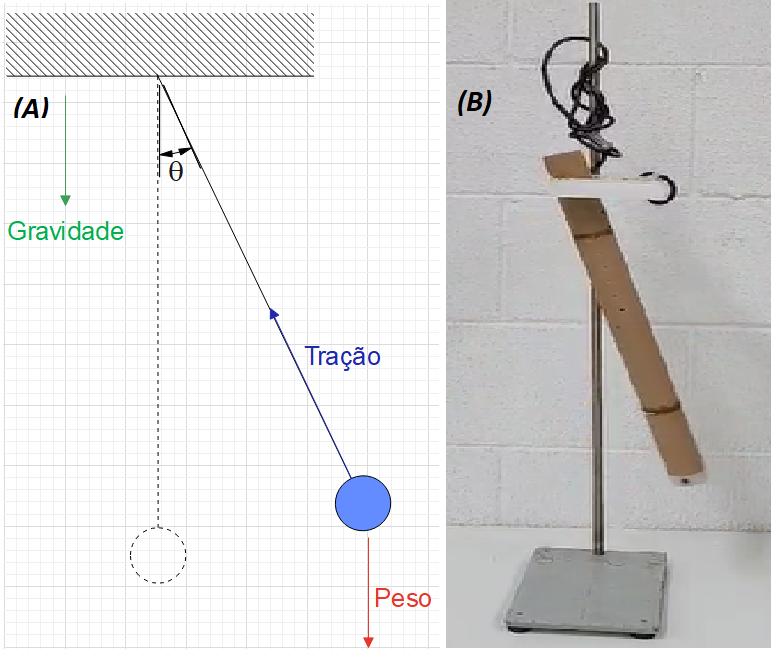
\includegraphics[scale=0.5]{pendulo.png}
    \caption{COLOCAR IMAGEM DO TRACKER AQUI!!!!!}
    \label{fig:enter-label}
\end{figure}
\pagebreak
\section*{Resultado}
\qquad 
\section*{Discussão}
\section*{Conclusão}
\section*{Referências}
“F 229 — Física Experimental II, Guia de Laboratório”, Coordenador: Pierre-Louis de Assis, versão 1.1.0 (outubro 2022) \\ \ \\ 
\qquad Hollow Cylinder Moment of Inertia. Disponível em: https://amesweb.info/inertia/hollow-cylinder-moment-of-inertia.aspx\\ \ \\ 
NUSSENZVEIG, H. Moysés. Curso de física básica 2: Fluidos, oscilações e ondas, calor. 5.ed. São Paulo: Blucher, 2013.
\section*{Apêndice A: Dados experimentais e incertezas}

\end{document}